\chapter{Process Reflections}
\label{chap:process-reflections}

\section{Main Results}
\label{sec:main-result}

The headline benchmark from the scientific article compares the proposed \texttt{ctc\_simple} against the National Library of Norway's best TrOCR variants. The strongest TrOCR variant (\texttt{trocr\_smi\_synth}) sets the SOTA at \trocrBestCER{}\% CER (\trocrBestCharAcc{}\% character accuracy\footnote{Character accuracy is measured directly and does not equal $100-\text{CER}$, since CER counts insertions as well as substitutions and deletions.}), with \texttt{ctc\_simple} within \cerGap{}~pp at \ctcCER{}\% CER (\ctcCharAcc{}\% character accuracy). On efficiency the picture flips. The lightweight model runs roughly \speedupFactor{}$\times$ faster on the same CPU and is \sizeRatio{}$\times$ smaller (\ctcSize{}~MB vs.\ \trocrSize{}~MB), which is decisive for heritage digitisation. At \ctcTime{}~s per image a CPU pushes about \ctcThroughputK{},000 images per hour, so a million page corpus runs in under \millionPagesCtcHours{} hours where TrOCR would need around \millionPagesTrocrDays{} days, and the small footprint fits edge devices that TrOCR cannot.

Table~\ref{tab:extended_results} reports the complete benchmark across all 11 models: the seven TrOCR variants released by the National Library of Norway, the proposed \texttt{ctc\_simple}, and the three ImageNet-pretrained CTC backbones that failed to converge. Extended comparison plot from the scientific article in Figure~\ref{fig:comparison1}.

\begin{table}[h]
\centering
\caption{OCR benchmark on \testSamples{} test samples: all 7 TrOCR variants from the National Library of Norway, the proposed lightweight \texttt{ctc\_simple}, and the three ImageNet-pretrained CTC backbones that failed to converge. Bold marks the best value in each column. Lower CER/WER is better, higher Exact Match Accuracy is better.}
\label{tab:extended_results}
\small
\resizebox{\linewidth}{!}{%
\begin{tabular}{@{}llccccc@{}}
\toprule
\textbf{Model} & \textbf{Training Data} & \textbf{CER↓} & \textbf{WER↓} & \textbf{Exact↑} & \textbf{sec / img} & \textbf{Size} \\
 & & \textbf{(\%)} & \textbf{(\%)} & \textbf{(\%)} & & \textbf{(MB)} \\
\midrule
trocr\_smi\_synth & Smi+Synth & \textbf{\trocrBestCER{}} & \textbf{\trocrBestWER{}} & \textbf{42.08} & \trocrBestTime{} & $\sim$\trocrSize{} \\
\textbf{ctc\_simple} & Smi+Synth & \ctcCER{} & \ctcWER{} & 36.74 & \textbf{\ctcTime{}} & \textbf{\ctcSize{}} \\
trocr\_smi\_pred\_synth & Smi+Pred+Synth & \trocrSmiPredSynthCER{} & \trocrSmiPredSynthWER{} & \trocrSmiPredSynthWordAcc{} & \trocrSmiPredSynthTime{} & $\sim$\trocrSize{} \\
trocr\_smi\_nor\_pred\_synth & Smi+Nor+Pred+Synth & \trocrSmiNorPredSynthCER{} & \trocrSmiNorPredSynthWER{} & \trocrSmiNorPredSynthWordAcc{} & \trocrSmiNorPredSynthTime{} & $\sim$\trocrSize{} \\
trocr\_smi & Smi only & \trocrSmiCER{} & \trocrSmiWER{} & \trocrSmiWordAcc{} & \trocrSmiTime{} & $\sim$\trocrSize{} \\
trocr\_smi\_pred & Smi+Pred & 24.82 & 63.06 & 16.32 & 11.730 & $\sim$350 \\
trocr\_smi\_nor & Smi+Nor & 25.84 & 66.62 & 13.17 & 12.890 & $\sim$350 \\
trocr\_smi\_nor\_pred & Smi+Nor+Pred & 26.43 & 64.21 & 17.08 & 11.759 & $\sim$350 \\
ctc\_vgg19 & Smi+Synth & 71.86 & 97.89 & 0.00 & 0.055 & $\sim$550 \\
ctc\_vgg16 & Smi+Synth & 73.94 & 98.81 & 0.00 & 0.044 & $\sim$550 \\
ctc\_resnet50 & Smi+Synth & 75.30 & 98.64 & 0.00 & 0.034 & $\sim$100 \\
\bottomrule
\end{tabular}%
}
\footnotesize
$^*$Training-data tags: \texttt{smi}=S\'{a}mi data, \texttt{nor}=+Norwegian, \texttt{pred}=+auto-transcribed, \texttt{synth}=+synthetic pre-training. 
\end{table}

The three CTC variants with ImageNet pretrained backbones (\texttt{ctc\_vgg16}, \texttt{ctc\_vgg19}, \texttt{ctc\_resnet50}) all failed to converge to usable performance ($>$69\% CER, $\sim$0\% exact match accuracy) despite sharing the projection layer and CTC head with the working \texttt{ctc\_simple} model. None of the four variants uses a recurrent encoder, so the backbone is the only difference. Two distinct training signatures emerged (Figure~\ref{fig:training-curves}). The VGG pair underfits on both ends, training loss drops from 0.81 only to $\sim$0.60 over around 60 epochs and validation CER never breaks the 0.72 barrier. ResNet50, conversely, fits the training set aggressively, train loss collapses from 0.80 to 0.23 in 37 epochs while validation CER stays unchanged at 0.73 and validation loss bounces upward (a likely sign of overfitting). The same underlying outcome appears in both: the pretrained features exposed to the CTC head did not generalise to character level prediction on this dataset.

\begin{figure}[h]
\centering
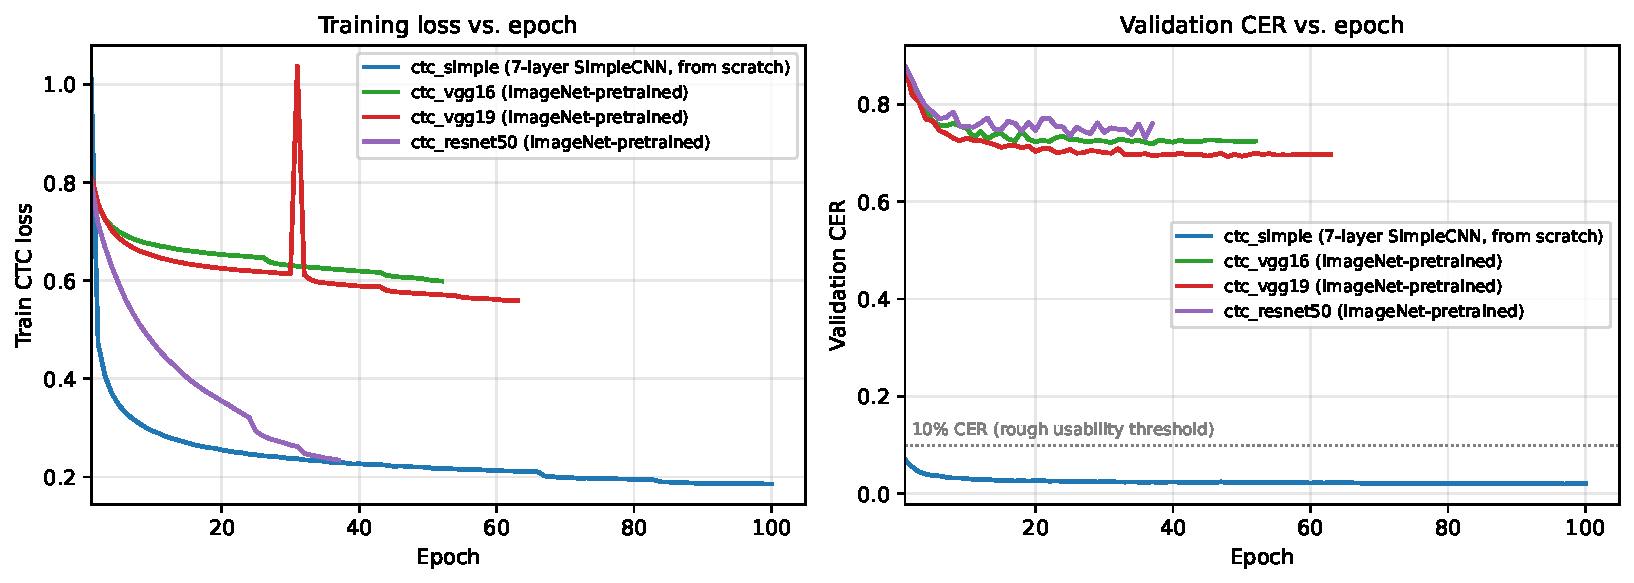
\includegraphics[width=\linewidth]{figures/training_curves.pdf}
\caption{Training dynamics of \texttt{ctc\_simple} (blue) vs.\ the ImageNet pretrained CTC variants \texttt{ctc\_vgg16} (green), \texttt{ctc\_vgg19} (red) and \texttt{ctc\_resnet50} (purple). Left: training CTC loss, \texttt{ctc\_simple} converges to near zero, the VGG pair underfits, ResNet50 overfits. Right: validation CER, \texttt{ctc\_simple} reaches below 10\% while all pretrained variants stay stuck around 0.70 until early stopping.}
\label{fig:training-curves}
\end{figure} 

\texttt{ReduceLROnPlateau} repeatedly halved the learning rate with no resulting improvement in validation CER for any of the failed variants. This behaviour rules out one obvious reason that learning rate was too high or of gradient instability, because both would normally respond to a smaller step size. The pretrained backbones were already updating at a very low effective learning rate (a base of $3{\times}10^{-5}$, further scaled by 0.1 on the backbone to give $3{\times}10^{-6}$), so too little learning might have been the issue. The VGG pair illustrates this, with training loss barely moving ($0.81 \rightarrow 0.60$), which is what one would expect if the backbone is learning too slowly to adapt. ResNet50 reveals something else. Training loss falls sharply from $0.80$ to $0.23$ over 37 epochs while validation CER stays flat. This indicates the head had enough  capacity to fit and memorise the pretrained features, but those features did not transfer to the character-level recognition task in the first place.

Concrete prediction examples for \texttt{ctc\_simple} on the in domain test-set are shown in Figure~\ref{fig:report-predictions}.
Full results comparison in Figure~\ref{fig:comparison1}. 
\begin{figure}[h]
\centering
\small
\begin{tabular}{p{0.93\linewidth}}
\toprule
\textbf{(a) Correct transcription (CER $=$ 0\%)} \\
\midrule

\includegraphics[width=\linewidth]{figures/correct1.jpg} \\
\textbf{Ground truth:} \textit{julev- ja davvis\'{a}migielagiiguin ja s\'{a}miiguin geat eai} \\
\textbf{Prediction:} \textit{julev- ja davvis\'{a}migielagiiguin ja s\'{a}miiguin geat eai} \\
\midrule
\textbf{(b) Diacritical error (CER $=$ 8.3\%)} \\
\midrule

\includegraphics[width=\linewidth]{figures/diacritical_errors_new.jpg} \\
\textbf{Ground truth:} \textit{ođđasis eal\'{a}skahttojuvvon) Suohkana h\'{a}lddahusla\v{s}} \\
\textbf{Prediction:} \textit{oddasis eal\'{a}skahttojuvvon) Duohkama h\'{a}lddahusla\v{s}} \\
\footnotesize \textit{Note: ođđasis $\rightarrow$ oddasis is the classic đ$\rightarrow$d error (the stroke is missed by the model).} \\
\midrule
\textbf{(c) Uppercase error (CER $=$ 29.6\%)} \\
\midrule

\includegraphics[width=\linewidth]{figures/uppercase_errors.jpg} \\
\textbf{Ground truth:} \textit{FYLKKAGIELDDAIGUIN. FINNM\'{A}RKKU FYLKKAGIELDDAS LEA \'{A}IGUMU\v{S}\v{S}IEHTADUS S\'{A}MI} \\
\textbf{Prediction:} \textit{FYLKKAGIELDDAIGUI0. F1O0m\'{A}RKKU FYLKKAGIELDDAs LEA \'{A}IGUmU\v{S}e} \\
\footnotesize \textit{Note: all uppercase lines are rare in the training distribution. The model frequently slips into mixed case or substitutes letters with visually similar digits.} \\
\bottomrule
\end{tabular}
\caption{CNN-CTC predictions illustrating the model predictions. (a) most lines are accurately transcribed, (b) diacritical strokes are the most common error, (c) all uppercase lines, rare in the training distribution, are by far the worst case.}
\label{fig:report-predictions}
\end{figure}

\begin{figure}[h]
\centering

\includegraphics[width=\linewidth]{figures/benchmark_comparison2.png}
\caption{Test set CER, WER, and exact match accuracy across 11 models (7 TrOCR variants, the lightweight CNN-CTC, and 3 failed ImageNet pretrained backbones). Lower values are better for CER and WER, higher values are better for exact match accuracy.}
\label{fig:comparison1}
\end{figure}

\section{Out of Domain Generalisation}
\label{sec:ood}

The out of domain evaluation on synthetic renderings of Turi's \turiYear{} \textit{Muitalus s\'{a}miid birra} produced rather surprising results. In domain, TrOCR has the best accuracy at \trocrSynthHFCER{}\% CER on the Spr\r{a}kbanken validation samples alone, against \ctcCER{}\% for \texttt{ctc\_simple}. 

On the historical text test set, TrOCR degrades by \trocrSynthDeltaCER{}~pp (\trocrSynthHFCER{}\% $\rightarrow$ \trocrSynthBookCER{}\%) while \texttt{ctc\_simple} is essentially flat (\ctcCER{}\% $\rightarrow$ \ctcBookCER{}\%). One TrOCR variant (\texttt{trocr\_smi\_pred\_synth}) still beats \texttt{ctc\_simple} on raw book CER (\trocrPredSynthBookCER{}\%). After punctuation and whitespace normalisation, however, the lightweight model overtakes all TrOCR variants on book text (\ctcBookNormAcc{}\% normalised accuracy vs.\ \trocrSynthBookNormAcc{}\% for the best TrOCR) (See Figure~\ref{fig:dataset-comparison}).

The sample is small (\bookTestSamples{} pairs) so it's nowhere near conclusive, but it might suggest that the smaller model learns more transferable character level features and is less prone to overfitting to synthetic rendering artefacts in the training distribution.


\begin{figure}[h]
\centering

\includegraphics[width=\linewidth]{figures/per_dataset_comparison.png}
\caption{Per Dataset Comparison: Spr\r{a}kbanken validation split vs Turi's \turiYear{} \textit{Muitalus s\'{a}miid birra} benchmark results.
Exact match accuracy on the book set is near zero for all models due to punctuation and orthography discrepancies. Normalised accuracy is the more informative metric here.}
\label{fig:dataset-comparison}
\end{figure}



\section{Conjunction Based Sentence Splitting}
\label{sec:conjunction-split}

Splitting long inputs at North S\'{a}mi conjunction boundaries before OCR and rejoining the predictions afterwards dropped long sentence CER from \splitLongOriginalCER{}\% to \splitLongSplitCER{}\%, a \splitImprovement{}pp improvement, below the short sentence baseline of \splitShortCER{}\% removing the length accuracy degradation (paired test $p = \splitPValue{}$, Cohen's $d = \splitCohensD{}$, \splitImproveRate{}\% of split samples improved, none degraded). Sentence length against CER and improvements visible in Figure~\ref{fig:cer-vs-length}.

% oracle upper bound
It is worth mentioning that the splitter acts on the ground truth strings rather than on a input OCR prediction, which makes the reported numbers a best case scenario, for the deployable variant would have to detect conjunctions on a noisy data (where short tokens like \textit{ja} and \textit{go} may themselves be misrecognised) or fall back to whitespace based segmentation of the line image, both of which are expected to lose much of the stated \splitImprovement{}\,pp gain. In addition, each segment is re-rendered as a fresh clean synthetic line image before OCR, so the experiment idealises both the segmentation \emph{and} the image quality, further inflating the reported upper bound.


\begin{figure}[h]
\centering

\includegraphics[width=\linewidth]{figures/cer_vs_length.pdf}
\caption{Character Error Rate of the lightweight CNN-CTC against the sentence length and the CER change after the split experiment.}
\label{fig:cer-vs-length}
\end{figure}


\section{End to End Pipeline}
\label{sec:e2e}

After passing the OCR predictions into TartuNLP's North S\'{a}mi English machine translation API~\cite{tartunlp}. The output scored BLEU \bleuScore{}, chrF \chrfScore{}~\cite{popovic2015chrf} and TER \terScore{}\% on the out of domain parallel set.

The moderate translation quality reflects how OCR errors propagate downstream, and the effect is even more pronounced for agglutinative languages. At \ctcCER{}\% CER, many of the relatively minor character errors land on the word endings that signal a noun's grammatical role or attach meaning like tense, number, and possession, rather than on the core part of the word that carries its meaning. Because these endings encode how words relate to one another in a sentence, a single dropped character can flip way the whole clause is read and degrade MT accuracy further. The results do not yield a fully fluent automatic translation, but they show that an end to end pipeline is in fact viable, even if for now it is best suited to simple downstream tasks such as archival indexing or content discovery rather than complete translation.


\begin{figure}[h]
\centering

\includegraphics[width=\linewidth]{figures/tartu_nlp_translation.png}
\caption{The TartuNLP translation web interface, available at \protect\url{https://translate.ut.ee/}. The same backend is used programmatically in the end to end pipeline via TartuNLP API.}
\label{fig:tartu-nlp}
\end{figure}


\section{Applications}
\label{sec:applications}
The lighweight OCR models allows multiple application cases. The community driven preservation projects (small archives, local museums, language enthusiasts) typically operate without dedicated GPU or many resources at hand. A model that runs on a phone or a small laptop and fully offline, would remove the deployment friction that would otherwise keep these efforts away from being realized.  The lightweight model is realistic as the OCR layer in a search and indexing pipeline over million page historical corpora in archival context, or as a back-end for educational tools that need to react to text in real time (for example, mobile flashcards that take a photo of a S\'{a}mi book page). Lastly, a combination of the CNN-CTC model with a generative model (a Stable Diffusion inpainting pipeline) for joint recognition and reconstruction of occluded text. Figure~\ref{fig:report-applications} shows the proof of concept output, an artificially occluded North~S\'{a}mi line is fed through OCR and inpainting, producing both a transcription and a plausible reconstruction of the original image with damaged text. This kind of pipeline becomes possible only when each component is small and fast enough to run together on an embedded device, useful in self driving settings (partially obscured road signs), in retail (damaged product labels), or in next generation robotic assistants where text in the visual scene must be interpreted continuously.

\begin{figure}[h]
\centering
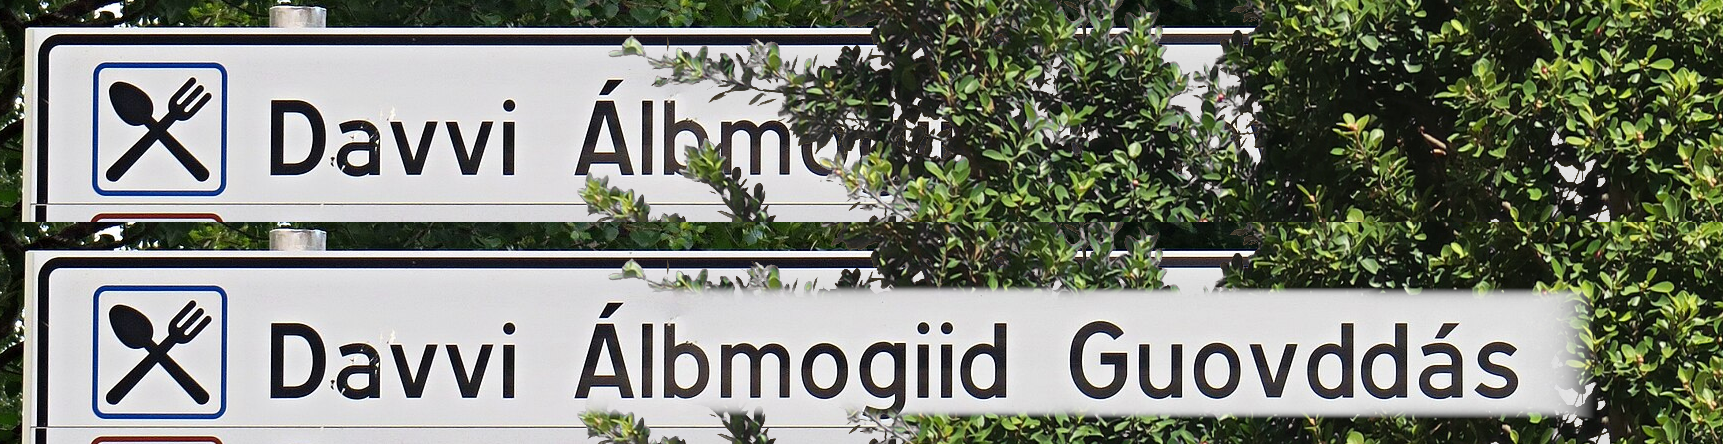
\includegraphics[width=\linewidth]{figures/reconstruction.png}
\caption{Proof of concept damaged text reconstruction combining \texttt{ctc\_simple} with a generative inpainting model on an artificially occluded North~S\'{a}mi line. The pipeline produces both a transcription and a reconstructed image. Enabled by the lightweight footprint, out of reach for the TrOCR baseline. Demonstrated as a future work direction in the IISA paper.}
\label{fig:report-applications}
\end{figure}

\section{Future work}
\label{sec:future-work}

The project leaves several questions unanswered and opens multiple options for future work. 
The main question still open to investigation is robustness to physical degradation. The entire benchmark in this thesis is conducted on synthetic renderings, and collecting and annotating a small corpus of real scanned S\'{a}mi documents (with realistic artefacts such as paper texture, ink bleed, skew and historical fonts) would validate the project's applicability.
The CTC model is weakest on rare inflected forms. Integrating Giellatekno's morphological analyser~\cite{moshagen2014} as a post correction layer, for instance by rescoring the top $k$ CTC hypotheses against a finite state lexicon, could selectively repair exactly the errors that propagate worst into downstream MT, without enlarging the deployed model.
Next, as \texttt{ctc\_simple} works on line level, applying Layout analysis and full page processing by pairing it with a lightweight line and region detector would elevate its usability from transcribing a cropped line to being able to process a full page, which matters for archival use cases.
Furthermore, it would be beneficial to check if the same approach works on different languages. Retraining the same architecture on other Uralic varieties (Inari, Skolt, Lule S\'{a}mi) or on unrelated low resource scripts would test if the same choices generalise, and if the same ImageNet pretraining issue appears. Finally, because the current decoder is purely greedy, showing the model's confidence in its predictions would increase the model's transparency.



\section{Conclusion}
\label{sec:conclusion}

The honest answer to the research question from (Section~\ref{sec:research-question}) is: \textbf{partially}. Depandant on the specific aspect of the question, the answer ranging from  yes to inconclusive.
\begin{itemize}
  \item \textbf{Deployment:} The size and speed advantage of \texttt{ctc\_simple} over the strongest TrOCR baseline is the difference between a million page archive processable in hours on widespread available hardware and one that would take days, and the difference between an OCR model that fits on a phone and one that does not. Unequivocally addressing the goal as achieved.
  \item \textbf{Accuracy:} On the in domain synthetic benchmark, \texttt{ctc\_simple} trails the best TrOCR variant by only \cerGap{}\,pp in CER, closer than the size difference would predict, and on the out of domain historical text subset it actually overtakes TrOCR on normalised accuracy. However, for an agglutinative language those few percentage points make a huge difference. The downstream OCR$\rightarrow$MT pipeline might be enough for archival indexing or content discovery but not for fluent automatic translation. Answering the question as yes but with few caveats.
  \item \textbf{Validation:} The entire evaluation in this thesis is conducted on synthetic renderings, with \bookTestSamples{} out of domain samples drawn from a single 1910 book. The model's behaviour on real scanned documents, with realistic paper, ink and degradation artefacts, has not been tested. As of now, the question remains unanswered.
\end{itemize}

The six contributions stated in Chapter~\ref{chap:goals} are all delivered: a lightweight CNN-CTC architecture, a systematic 11 model benchmark, a Sustainable AI footprint argument, an end to end OCR$\rightarrow$MT pipeline, a linguistically motivated conjunction splitting method, and a discussion of education, AI~\&~NLP and robotics applications. The three ImageNet pretrained CTC baselines did not converge, so the within CTC comparison is partial, the out of domain set is small, and no real scan data was used. 
